\documentclass{beamer}
\usepackage{mathtools}
\usepackage{hyperref}
\usepackage{breakurl}
\usepackage{verbatim}
\title{Parallelized Attacks on Elliptic Curve Discrete Logarithm Problem}
\author{Qin ZHOU, Liang XIA \\
fatestudio@gmail.com, liangxia2006@gmail.com}
\institute{University of California, Santa Barbara}
\date{March 5, 2013}
\usetheme{Berlin}
\begin{document}
  \begin{frame}
  	\titlepage
  	%\insertframenumber/ %\inserttotalframenumber
  \end{frame}
  
  \begin{frame}
    \frametitle{Elliptic Curve (on Finite Field $p$)}
    \begin{itemize}
    \item Elliptic Curve $E: y^2 = x^3 + Ax + B\ (mod\ p)$\\
	\item Nodes: $P = (x, y) \in E, x, y \in Z_p^ {\ast}$\\ 
	
	\item Define addition operation on EC nodes:\\ 
	$P_1 + P_2 = (x_1, y_1) + (x_2, y_2) = P_3 = (x_3, y_3) $\\
	
	$x_3 = m^2 - x_1 - x_2$ \\
	$y_3 = m(x_1 - x_3) - y_1$\\
	$m = \left\{
	\begin{array}{l l}
    	(y_2 - y_1)/(x_2 - x_1) & \quad P_1 \neq P_2\\
    	(3x_1^2 + b)/(2y_1) & \quad P_1 = P_2
  	\end{array} \right.$\\
  	If the slope $m$ is infinite, then $P_3 = \infty$. There is one additional law: $\infty + P = P$ for all points $P$\\
  	\item Nodes set $\mathbb{P}$ with addition operation $+$ forms a \alert{Abelian Group}
	\end{itemize}
  \end{frame}
    
  \begin{frame}
  	\frametitle{Addition: $P_1 + P_2 = P_3\ (P + Q = R)$}
  	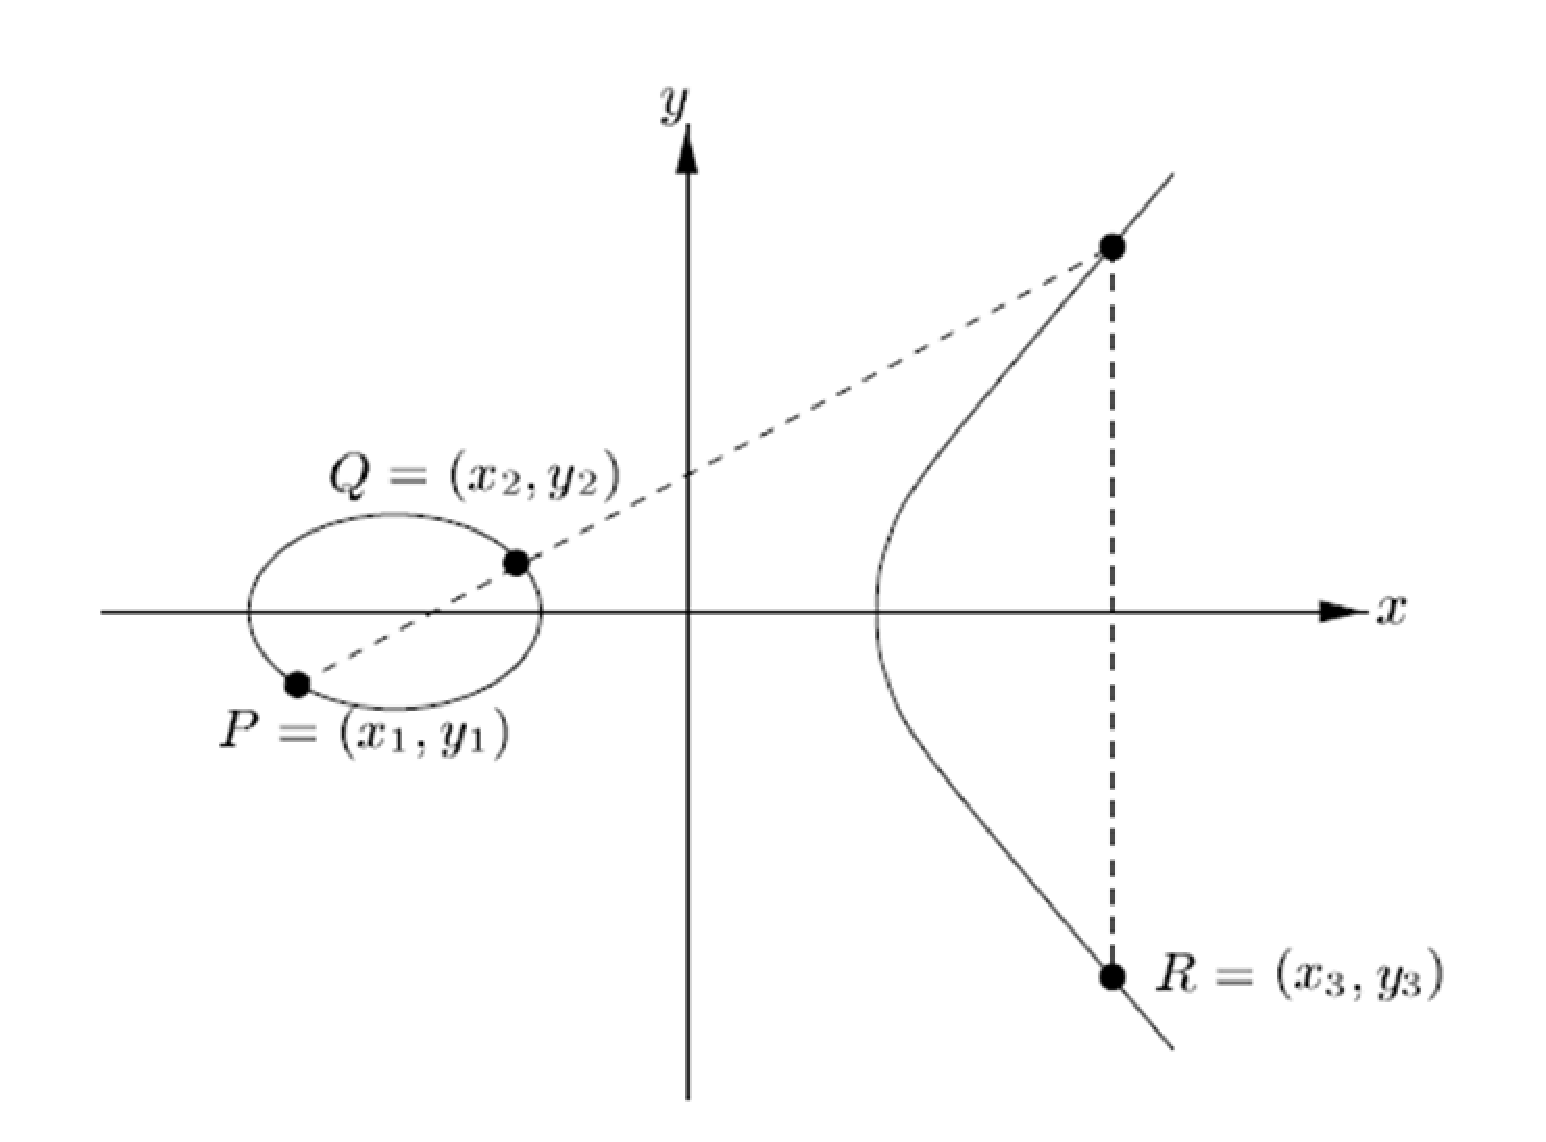
\includegraphics[scale=0.3]{p1p2.eps}
  \end{frame}
  
  \begin{frame}
  	\frametitle{Addition: $P + P = 2P$}
  	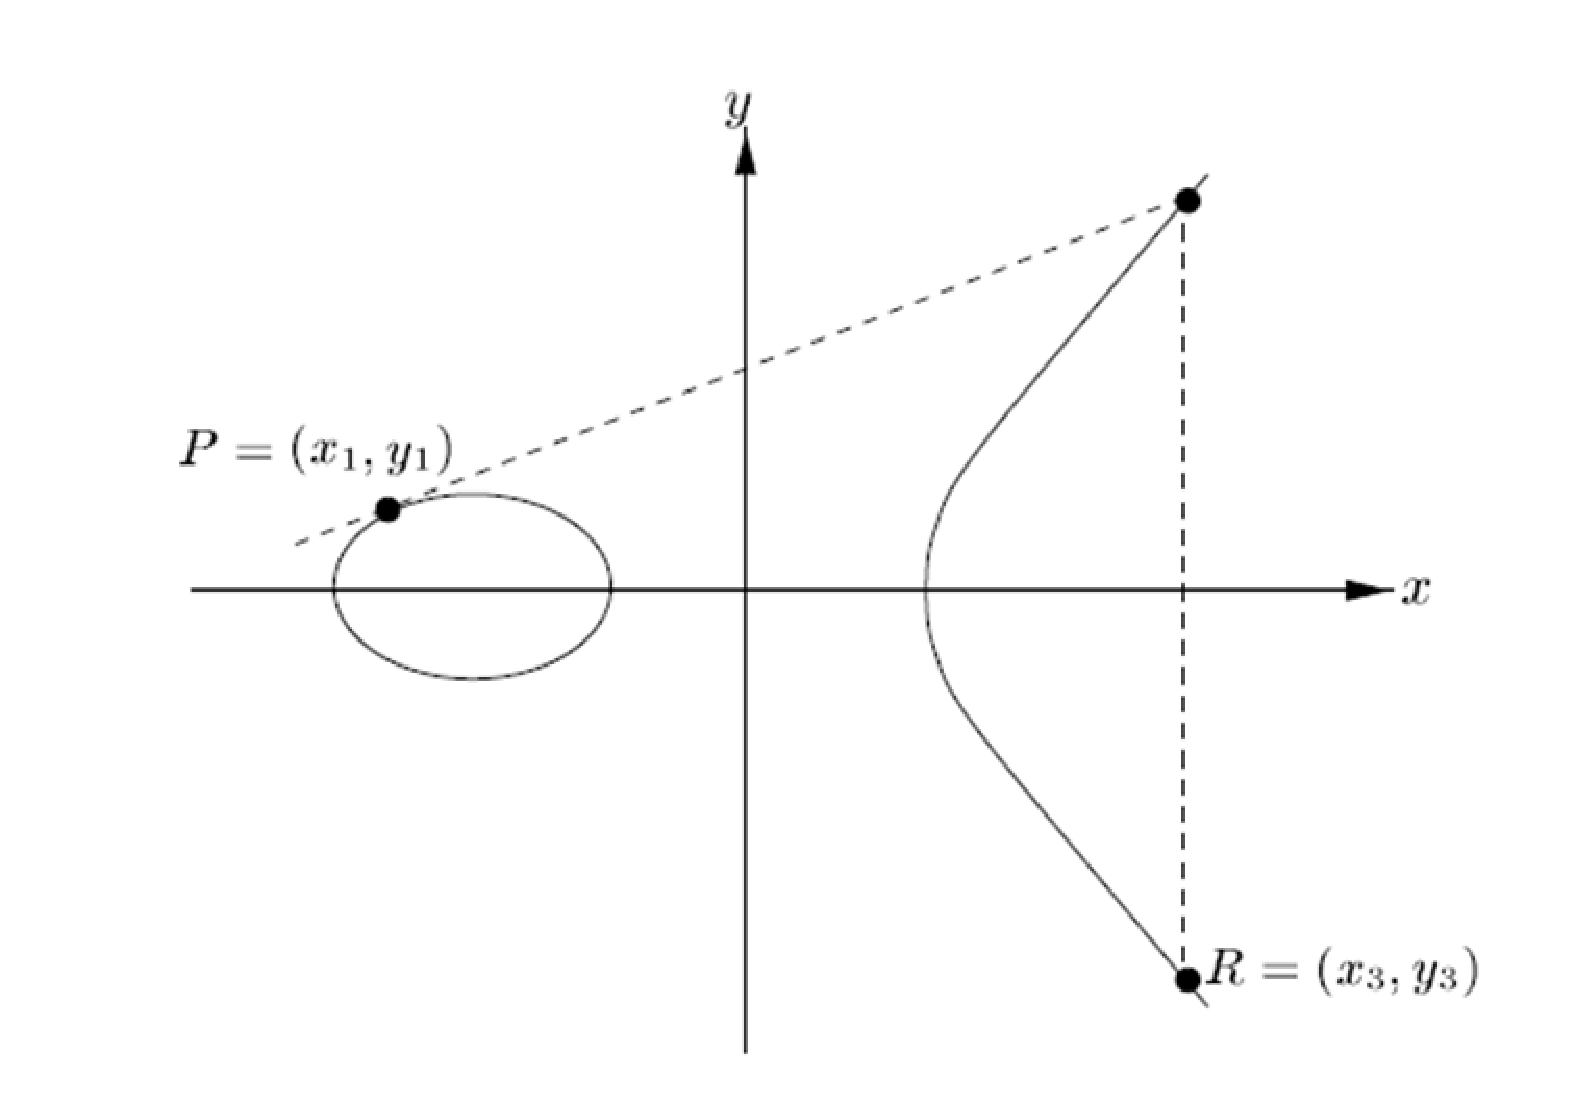
\includegraphics[scale=0.3]{2p.eps}
  \end{frame}
  
  \begin{frame}
  	\frametitle{Elliptic Curve Discrete Logarithm Problem (ECDLP)}
  	\begin{itemize}
		\item If we have a curve $E$, a node $P$, and a number $k$, calculate $kP$ is easy: $(k, P) \rightarrow kP$\\
  		e.g. Using \textbf{binary method of exponentiation} to compute $254P$:\\
  		$P\xrightarrow{d}2P\xrightarrow{a}3P
  		\xrightarrow{d}6P\xrightarrow{a}7P
  		\xrightarrow{d}14P\xrightarrow{a}15P
  		\xrightarrow{d}30P\xrightarrow{a}31P
  		\xrightarrow{d}62P\xrightarrow{a}63P
  		\xrightarrow{d}126P\xrightarrow{a}127P
  		\xrightarrow{d}254P$\\
  		\item However, If we have $kP$ and $P$, get $k$ is \alert{hard}: $(kP, P) \not\rightarrow k$
  	\end{itemize}
  \end{frame}
  
  \begin{frame}
  	\frametitle{Applications of ECDLP}
  	\begin{itemize}
  		\item Example: Elliptic Curve Diffie Hellman (ECDH)\\
  		Share a secret \alert{$k_ak_bP$} between Alice and Bob preventing Eve
\begin{align*}
& \text{Alice} & \quad & \text{Bob} & \\
& \text{private key:} k_a & \quad & \text{private key:} k_b & \\
& \text{public key:} k_aP & \quad & \text{public key:} k_bP & \\
& k_aP \xrightarrow{to Bob} & \quad &\\
& & \quad & \xleftarrow{to Alice} k_bP & \\
& \text{Shared key:} k_a*k_bP=k_ak_bP & \quad  &\text{Shared key:} k_b*k_aP=k_ak_bP &
\end{align*}
  		\item Other Examples: EC Digital Siganiture Authentication (ECDSA), EC ElGamal
	\end{itemize}
  \end{frame}
  
  \begin{frame}
  	\frametitle{Why use Elliptic Curve?}
	\begin{itemize}
		\item Using much less bits while achieving the same Level security compared to RSA (160 bits of ECC $\approx$ 1024 bits of RSA)\\
		\item Less bits means less bandwidth usage and better performance  
	\end{itemize}	  	
  \end{frame}
  
  \begin{frame}
  	\frametitle{Attacking ECDLP}
  	\framesubtitle{Attacking Methods}
  	\begin{itemize}
  		\item 1. Exhaustive Key Search (Time:$O(n)$, $n$ is the order of $P$; Space:$O(1)$)\\
  		\item 2. Baby Step, Giant Step (Time:$O(\sqrt{n})$; Space:$O(\sqrt{n})$)\\
  		\item 3. Pollard's $\rho$ Method (Time:$O(\sqrt{\pi n/2})$; Space:negligible)\\
  		\item 4. \alert{Distributed version of Pollard's $\rho$ algorithm} (Time:$O(\sqrt{\pi n/2}/2m)$; Space:negligible)\\
  		\item 5. Pohlig-Hellman Method (Need factoring, which is hard)\\
  		\item ...
  	\end{itemize}
  \end{frame}
  
\begin{comment}
  \begin{frame}
  	\frametitle{Pollard's $\rho$ Methods}
  	\begin{itemize}
  		\item Let $G$ denote a group of order $n$ and let $Q = dP$\\
		\item Partition $G$ into three sets $S_1, S_2, S_3 (\infty \not\in S_2)$\\
		\item Define the following random walk\\	
		$X_{i+1} = f(X_i) = \left\{
		\begin{array}{l l}
			Q + X_i & \quad X_i \in S_1\\
			2X_i	& \quad X_i \in S_2\\
			P + X_i & \quad X_i \in S_3
		\end{array} \right.$
  	\end{itemize}
  \end{frame}  

  \begin{frame}
  	\frametitle{Pollard's $\rho$ Methods}
  	Let $X_i = a_iP + b_iQ$, then\\
  	$a_{i+1} = \left\{
		\begin{array}{l l}
			a_i & \quad x_i \in S_1\\
			2a_i\(mod\n)	& \quad x_i \in S_2\\
			a_i + 1\(mod\n) & \quad x_i \in S_3
		\end{array} \right.$\\
	and \\
	$b_{i+1} = \left\{
		\begin{array}{l l}
			b_i + 1\(mod\n) & \quad x_i \in S_1\\
			2b_i\(mod\n)	& \quad x_i \in S_2\\
			b_i & \quad x_i \in S_3
		\end{array} \right.$\\
	
  	
  \end{frame} 
  
  \begin{frame}
  	\frametitle{Framework of Parallelized Attacks}
  	%Need a graph!!
  	
  	
  \end{frame}
\end{comment}
  
  \begin{frame}
  	\frametitle{Pollard $\rho$ Method}
  	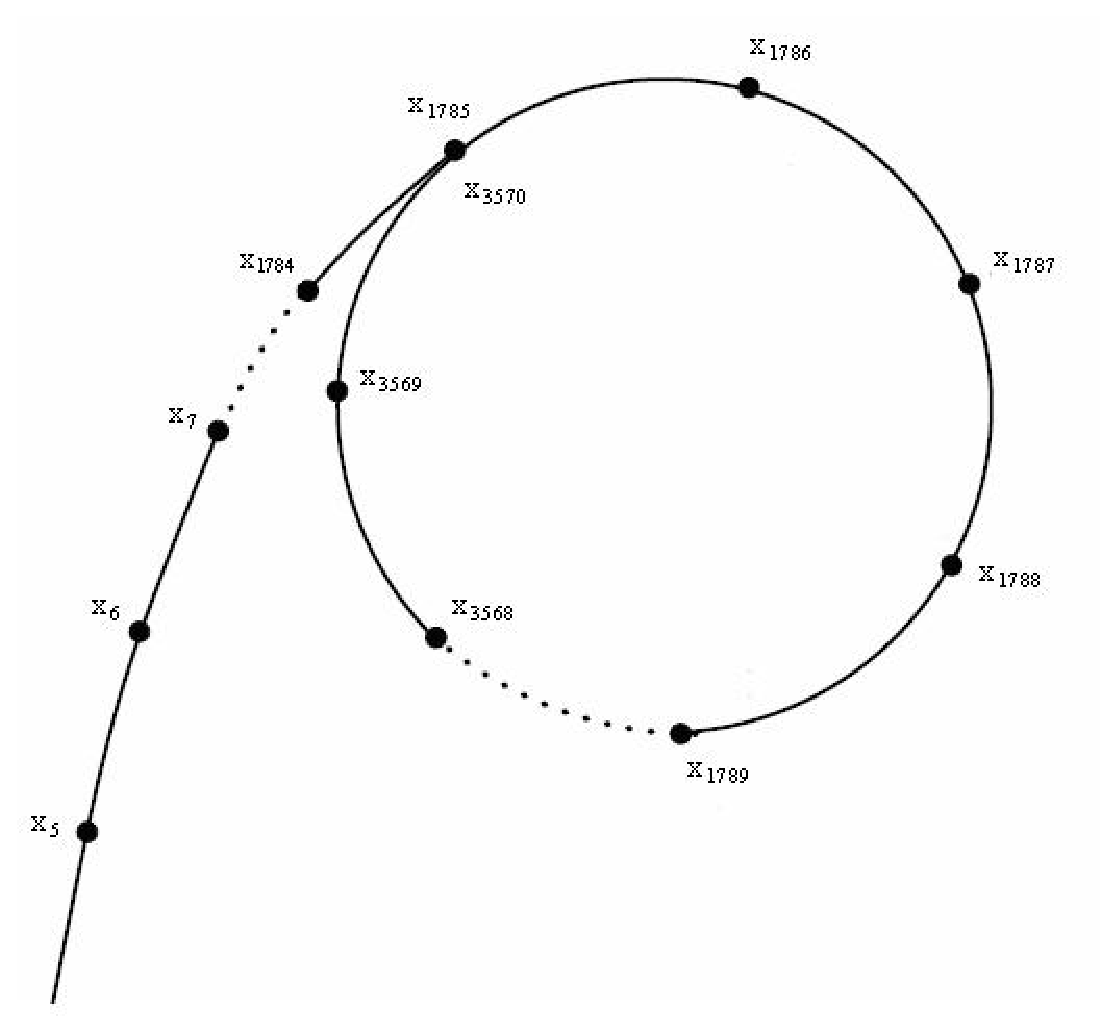
\includegraphics[scale=0.4]{rho.eps}
  \end{frame}
  
  \begin{frame}
  	\frametitle{Parallel Pollard Rho (van Oorschot and Wiener)}
  	\begin{itemize}
  		\item With $m$ processors, $m$ pseudo-random walks starting at\\
  		$X_o^{(i)} = a_iP + b_iQ$\\
  		\item Each processor need to compute $O(\sqrt{\pi n/2}/m)$ iterations\\
  		\item Central server need to store all $O(\sqrt{\pi n/2})$ points\\
  		\item Define distinguished points $S_D \subset G$ and $\theta = |S_D|/|G|$\\
  		\item Processors only send distinguished points to central server\\
  		$O(\frac{\sqrt{\pi n/2}}{m} + \frac{1}{\theta})$ time \qquad $O(\theta\sqrt{\pi n/2})$ space
  	\end{itemize}
  \end{frame} 
  
  \begin{frame}
	\frametitle{Challenges}
	\begin{itemize}
		\item Build everything from scratch (because standardized Elliptic Curves are too large to break)\\
		\item Efficiently find the order of $G$\\
		\item Build parallelized attacking framework
	\end{itemize}	  
  \end{frame}
  
  \begin{frame}
  	\frametitle{Steps of implementation}
  	\begin{itemize}
  		\item Set the maximum number of bits $N$. All numbers in this implementation are smaller than $2^N$ \\
  		\item generate $A$, $B$ and a prime $p$ to form a Elliptic Curve\\
  		\item randomly find a base $G$\\
  		\item \alert{get the order of this $G\ (nG = \infty)$}\\
  		\item choose a random $k$ that $0 \leq k < n$ as the private key and compute $kG$ as the public key\\
  		\item implement attacks	
  	\end{itemize}
  \end{frame}
  
  \begin{thebibliography}{}
  	\begin{frame}
  	\frametitle{Reference}
	\bibitem{CERTICOM} "Certicom ECC Challenge", \url{http://www.certicom.com/images/pdfs/cert_ecc_challenge.pdf}
	\bibitem{RFC6090} D. McGrew, K. Igoe and M. Salter, "Fundamental Elliptic Curve Cryptography Algorithms", RFC6090
    \bibitem{DH1976} Diffie, W. and M. Hellman, "New Directions in
                Cryptography", IEEE Transactions in Information
                Theory IT-22, pp. 644-654, 1976.

    \bibitem{E1985} ElGamal, T., "A public key cryptosystem and a signature
                scheme based on discrete logarithms", IEEE Transactions
                on Information Theory, Vol. 30, No. 4, pp. 469-472,
                1985.
  	\end{frame}
  
  	\begin{frame}
  	\frametitle{Reference}
	\bibitem{ECC Book} L. C. Washington, "Elliptic Curves Number Theory and Cryptography", Second Edition, 2008
  	\bibitem{ReHard} Junfeng Fan, el, "Breaking Elliptic Curve Cryptosystems using
Reconfigurable Hardware", 2010
	\bibitem{ECC2K} DV Bailey, "Breaking ECC2K-130", 2010  
	\end{frame}
  \end{thebibliography}
\end{document}